% README
% ------
% apt install texlive-full texlive-science
% thieu gi thieu apt search <cai bi thieu> hoac tra google
% sau do dien vao cac file input va compile file main
\documentclass{hust}
\usepackage[utf8]{vietnam}
\usepackage{graphicx}
\usepackage[acronym,nonumberlist]{glossaries}
\newacronym{CF}{CF}{Collaborative Filtering}
\newacronym{MFCF}{MFCF}{Matrix factorization collaborative filtering}

\graphicspath{ {./images/} }
\lfoot{Luong Tuan Linh - 20152186 - IS1 K60}

\makeglossaries

\begin{document}

\thispagestyle{empty}

\thisfancypage{
  \setlength{\fboxrule}{1pt}
  \doublebox}{}
\begin{center}

{\setstretch{1.4}
. \\
{\fontsize{12}{12}\fontfamily{cmr}\selectfont ĐẠI HỌC BÁCH KHOA HÀ NỘI\\VIỆN CÔNG NGHỆ THÔNG TIN VÀ TRUYỀN THÔNG}\\
\textbf{------------*******---------------}\\[1cm]

\includegraphics[width=3cm]{logo}
\centering
\\[1cm]
{\fontsize{25}{43}\fontfamily{cmr}\selectfont ĐỒ ÁN TỐT NGHIỆP}\\[0.1cm]
{\fontsize{17}{10}\fontfamily{cmr}\fontseries{b}\selectfont CHUYÊN NGÀNH HỆ THỐNG THÔNG TIN}\\[0.9cm]
{\fontsize{20}{26}\fontfamily{phv}\selectfont Đánh giá model hệ thống gợi ý}\\[2cm]

\begin{tabular}{l c l}
  \textbf{Họ và tên} & : & Lương Tuấn Linh \\ 
  \textbf{MSSV} & : & 20152186  \\ 
  \textbf{Lớp} & : & IS1 - K60  \\
  \textbf{GVHD} & : &  PGS.TS Thân Quang Khoát  \\
\end{tabular} \\[1.5cm]
}

\fontsize{17}{19}\fontfamily{cmr}\selectfont Hà Nội, Tháng 4 năm 2020
\end{center}
\pagebreak

\addcontentsline{toc}{chapter}{Thẻ nhiệm vụ tốt nghiệp}
\chapter*{Thẻ nhiệm vụ tốt nghiệp}
\section*{Thông tin sinh viên}

\begin{itemize}
\begin{multicols}{2}
\item \textbf{Họ và tên:} Lương Tuấn Linh
\item \textbf{Số điện thoại:} 0912201718
\item \textbf{Lớp học:} IS1 K60
\item \textbf{Email:} linh.lt152186@sis.hust.edu.vn
\item \textbf{Chương trình:} Kỹ Sư
\end{multicols}
% \item \textbf{Graduation Thesis conducted in:} Department of Computer Science - School of Information and Communication Technology.
\item \textbf{Thời hạn:} Từ tháng 1 năm 2019 đến tháng 6 năm 2020
\end{itemize}
\section*{Mục tiêu chính của đồ án}
\begin{enumerate}
    \item Nghiên cứu về thuật toán MFEA-II
    \item Nghiên cứu và áp dụng thuật toán MFEA-II trong huấn luyện mạng Nơ-ron
\end{enumerate}

\section*{Nhiệm vụ cụ thể của đồ án}
\begin{enumerate}
    \item Nghiên cứu về cấu trúc, cách thực hiện của thuật toán MFEA-II
    \item Áp dụng thuật toán MFEA-II vào tối ưu hóa mạng Nơ Ron có cấu trúc với các bộ dữ liệu UCI, các môi trường OpenAI gym
    \item Cài đặt thuật toán dưới dạng một thư viện để áp dụng giải quyết nhiều bài toán khác nhau
    \item Thực nghiệm, mô hình hóa, phân tích kết quả thu được
\end{enumerate}

\pagebreak

\section*{Cam kết của sinh viên}
Tôi là \textit{Hoàng Minh Quang} cam đoan rằng nội dung trong đồ án này là của tôi dưới sự hướng dẫn của PGS.TS Huỳnh Thị Thanh Bình.

Các đề xuất và kết quả trong đồ án này đều là xác thực và nguyên bản.
\begin{minipage}{0.5\textwidth}
.
\end{minipage}
\begin{minipage}[t]{0.5\textwidth}



\begin{center}
  \textit{Hà Nội}, Ngày 31 Tháng 3 năm 2020\\
  Tác giả đồ án\\[3cm]
  
  \textit{Hoang Minh Quang}
\end{center}
\end{minipage}
\subsection*{Xác nhận về mức độ hoàn thiện đồ án và cho phép đồ án được bảo vệ bởi giáo viên hướng dẫn}
.\dotfill \\
.\dotfill \\ 
.\dotfill \\ 
.\dotfill \\
\begin{minipage}{0.5\textwidth}
.
\end{minipage}
\begin{minipage}[t]{0.5\textwidth}

\begin{center}
  \textit{Hanoi}, Ngày 31 Tháng 3 năm 2020\\
  Người hướng dẫn\\[3cm]
  
  \textit{PGS.TS Huỳnh Thị Thanh Bình}
\end{center}
\end{minipage}

\pagebreak


\addcontentsline{toc}{chapter}{Lời cảm ơn}
\chapter*{Lời cảm ơn}
% Đồ án này sẽ không thể hoàn thiện nếu không có lời khuyên và sự hỗ trợ nhiệt tình mà tôi được nhận từ người hướng dẫn của tôi - PGS.TS Huỳnh Thị Thanh Bình. Mặc dù giáo sư bận rộn trong việc hỗ trợ nhiều nghiên cứu sinh, sinh viên, nhưng cô vẫn dành thời gian quý báu để giúp đỡ tôi nghiên cứu tốt hơn. Cùng với đó cô cũng đã tạo ra một môi trường nghiên cứu tuyệt vời để tôi và các sinh viên khác được cạnh tranh, cải thiện kết quả trong học tập và nghiên cứu. Tôi muốn bày tỏ lòng biết ơn của mình đến giáo sư Bình và chúc cô ngày càng thành công hơn trong công việc nghiên cứu, hỗ trợ sinh viên, cũng như thành công trong cuộc sống. 

% Qua 5 năm học tập và nghiên cứu tại đại học Bách Khoa Hà Nội, tôi muốn cảm ơn những người thầy cô với kiến thức và lòng nhiệt huyết đã tham gia giảng dạy, giúp định hình tri thức và niềm tin trong tôi như hiện tại.

% Đồ án này là tổng hợp của rất nhiều thời gian làm việc với mọi người trong Lab của tôi. Ở đây tôi được làm việc với nhiều sinh viên và các anh chị nghiên cứu sinh khác, tôi muốn cảm ơn họ những người đã khuyến khích tôi kiên trì với con đường hiện tại và trong tương lai đầy thử thách. Đặc biệt tôi muốn cảm ơn anh Thành, người anh tại Lab luôn hỗ trợ và động viên giúp tôi vượt qua những khó khăn khi bước vào công việc nghiên cứu.

% Cuối cùng, tôi muốn cảm ơn những người bạn đặc biệt tại lớp Việt Nhật K60C đã luôn ở đồng hành với tôi trong suốt 5 năm học tập dưới mái trường Bách Khoa Hà Nội. 

\setlength{\parindent}{4ex}
\setlength{\parskip}{1em}

Trong thời gian nghiên cứu đồ án, em đã nhận được nhiều sự giúp đỡ, đóng góp ý kiến và chỉ bảo nhiệt tình của thầy cô và bạn bè.\par

Em xin gửi lời cảm ơn chân thành đến thầy PGS.TS Thân Quang Khoát - trường Đại học Bách Khoa Hà Nội người đã tận tình hướng dẫn, chỉ bảo em trong suốt quá trình học tập, nghiên cứu đồ án.\par

Em cũng xin chân thành cảm ơn các thầy cô giáo trong trường Đại học Bách Khoa Hà Nội nói chung, các thầy cô giáo trong viện Công Nghệ Thông Tin và Truyền Thông nói riêng đã dạy dỗ cho em kiến thức về các môn học đại cương cũng như các môn chuyên ngành, giúp em có được cơ sở lý thuyết vững vàng và tạo điều kiện giúp đỡ em trong suốt quá trình học tập.\par

Cuối cùng, em xin chân thành cảm ơn bạn bè đã luôn hỗ trợ, giúp đỡ trong quá trình học tập và nghiên cứu.


% \begin{flushright}
% \begin{minipage}[t]{0.5\textwidth}
% \begin{center}
%   \textit{Hà Nội}, Ngày  tháng 3 năm 2020\\
  
%   \textit{Hoàng Minh Quang}
% \end{center}
% \end{minipage}
% \end{flushright}

\pagebreak

\addcontentsline{toc}{chapter}{Tóm tắt}
\chapter*{Tóm tắt}
More Text

Đồ án của tôi được xây dựng như sau:
\begin{itemize}
  \item \textbf{Chapter 1} Cung cấp thông tin, khái niệm tổng quan về thuật toán tiến hóa, cơ bản về thuật toán MFEA-II
  \item \textbf{Chapter 2} Giới thiệu về bài toán huấn luyện mạng Neural có cấu trúc Mô-đun (modular neural network) và huấn luyện mạng nơ ron trong học tăng cường
  \item \textbf{Chapter 3} Đề xuất hướng áp dụng thuật toán MFEA-II cho việc huấn luyện nhiều mạng Nơ-Ron có cấu trúc mô-đun với các lớp ẩn khác nhau và huấn luyện nhiều mạng nơ-ron cho các môi trường học tăng cường có liên quan đến nhau.
  \item \textbf{Chapter 4} Trình bày kết quả thực nghiệm, phân tích và đánh giá hiệu quả của giải thuật đã đề xuất
\end{itemize}

\pagebreak

% \begin{figure}
%     \includegraphics[width=\linewidth]{figures/other/abstract_vi}
% \end{figure}
% the best way is to create another vietnamese project with \usepackage[utf8]{vietnam}
% screenshot it
% then include here
\pagebreak


\addcontentsline{toc}{chapter}{Lời Nói Đầu}
\chapter*{Lời Nói Đầu}
Trong nhiều thập kỷ gần đây, tính toán tiến hóa là giải pháp tiên phong trong đó các thuật toán được lấy cảm hứng từ lý thuyết sinh học, đề xuất để....
....
...
...




\addcontentsline{toc}{chapter}{Thuật Ngữ}
\chapter*{Thuật Ngữ}
\printglossary[type=\acronymtype,style=long]

\fontsize{12}{16}\fontfamily{cmr}\selectfont

\begin{center}
\begin{tabular}{|l|l|l|l|}

\hline
\textbf{Acronym} & \textbf{Full terminology} & \textbf{Tiếng Việt} \\ \hline
    CF & Collaborative Filtering & Thuật toán tiến hóa\\ \hline

\end{tabular}    
\end{center}
\pagebreak

\addcontentsline{toc}{chapter}{Nội dung đã tìm hiểu}
\chapter*{Nội dung đã tìm hiểu}
Trong đồ án GR2 này, em đã tập trung tìm hiểu và học những kiến thức về hệ gợi ý (recommendation system). Những kiến thức đã tìm hiểu được bảo gồm những phần sau. Đầu tiên là sự cần thiết của recommendation system trong thời đại công nghệ hiện nay, cũng như những ứng dụng của recommendation system trong việc giới thiệu sản phẩm, dự đoán được sở thích của người dùng, ... Tiếp theo là những vấn đề vẫn còn gặp phải trong việc phát triển recommendation system. Cuối cùng là những phương pháp phát triển recommendation system bao gồm content-based và collaborative filtering.

\listoftables
\listoffigures

\newpage
\tableofcontents
\newpage

\acresetall

% % \chapter{Giới thiệu}
% \label{chap:introduction}

\section{Giải thuật tiến hóa}
\subsection{Động lực}
Motivation
\newpage
\subsection{Tối ưu}
optimization
\newpage
\subsection{Giải thuật tiến hóa cho tối ưu hóa liên tục}
continuous-optimization
\newpage
\subsection{Các tham số của thuật toán tiến hóa}
parameters
\newpage
\subsection{Phân loại thuật toán tiến hóa}
typical
\newpage
\section{Giải thuật tiến hóa đa nhiệm}
\subsection{Nền tảng và động lực của thuật toán tối ưu hóa đa nhiệm}
background
\newpage
\subsection{Tối ưu hóa đa nhiệm 1 - MFEAI}
mfeai
\newpage
\subsection{Tối ưu hóa đa nhiệm 2 - MFEAII}
mfeaii
\chapter{Tổng quan}
\label{chap:problem}
\section{Giới thiệu recommendation system}
Trong một vài thập kỷ gần đây, với sự phát triển của Youtube, Amazon, Netflix và rất nhiều các web service khác, recommendation system đang ngày càng trở nên quan trọng hơn. Từ các dịch vụ e-commerce (gợi ý cho người mua những sản phẩm mà họ có thể thích) cho tới quảng cáo online (gợi ý những quảng cáo phù hợp với từng người), recommendation system liên tục xuất hiện trong cuộc sống hàng ngày của mỗi người.

Nói chung, recommendation system là những thuật toán nhằm dự đoán mức độ quan tâm của 1 user đến 1 item (item ở đây có thể là phim để xem, những bài báo để đọc, những sản phẩm đang bán hay bất kì cái gì tùy thuộc vào từng lĩnh vực)

Recommendation system còn nắm vai trò thiết yếu trong một số lĩnh vực vì có khả năng tạo ra 1 lượng doanh thu vô cùng lớn nhờ vào mức độ chính xác và giúp nổi bật hơn so với các đối thủ cạnh tranh. Một minh chứng cho tầm quan trọng của recommendation system là, một vài năm về trước, Netflix đã tổ chức cuộc thi "Netflix prize" với mục đích để tìm được 1 recommendation system tốt hơn recommendation system hiện có với phần thưởng là 1 triệu đô.

Sau đây là 2 phương pháp đã tìm hiểu của recommendation system. Content-based recommendation system và collaborative filtering recommendation system.

% \newpage
\section{Utility Matrix}
Trong recommendation system có 2 thực thể chính là user và item. Mỗi user sẽ một độ quan tâm nhất định tới mỗi item. Mức độ quan tâm được gán cho một giá trị ứng với mỗi cặp user - item. Giả sử giá trị này được đo bằng giá trị user rate cho item, ta gọi giá trị này là rating. Khi đó, tập hệt các rating, bao gồm cả những giá trị chưa biết cần được dự đoán, được gọi là utility matrix.

Giả sử như ví dụ của utility matrix như hình dưới đây, user rate cho mỗi phim giá trị từ 1 đến 5, với 5 là rating tốt nhất. Khoảng trống thể hiện những phim mà user vẫn chưa rate. Những giá trị HP1, HP2, HP3 là phim Harry Potter 1, 2, 3, TW là Twilight, SW1, SW2, SW3 là Star Wars 1, 2, 3. User được thể hiện ở các chữ cái A đến D.

\begin{figure}[ht]
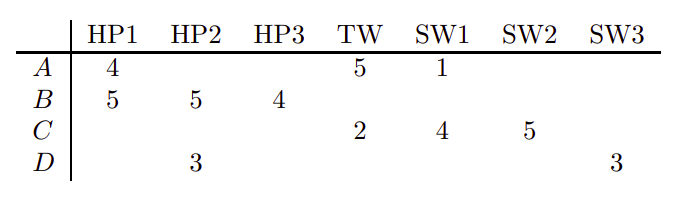
\includegraphics[width=\textwidth]{thesis/images/utility_matrix_2.png}
\caption{Utility Matrix}
\end{figure}

Thông thường, có rất nhiều user và item trong hệ thống, và mỗi user chỉ rate một số lượng ít các item hay không rate item nào. Do vậy trong utility matrix thường rất nhiều ô trống và những ô được điền là rất ít.

Rõ ràng càng nhiều ô được điền thì độ chính xác của hệ thống sẽ càng được cải thiện. Vì vậy các hệ thống luôn hỏi người dùng về sự quan tâm của họ tới sản phẩm, và muốn người dùng đánh giá càng nhiều sản phẩm càng tốt. Việc đánh giá sản phẩm không những giúp các người dùng khác biết được chất lượng sản phẩm mà còn giúp hệ thống biết được sở thích của người dùng, qua đỡ có thể quảng cáo hợp lý.

Nếu không có utility matrix thì gần như không thể gợi ý sản phẩm cho người dùng. Do vậy việc xây dựng utility matrix là việc rất quan trọng. Có 2 hướng tiếp cận phổ biến để xác định giá trị rating cho mỗi cặp user-item trong utility matrix. 

Hướng thứ nhất là nhờ người dùng rate sản phẩm. Ví dụ như Amazon luôn nhờ người dùng rate các sản phẩm của họ bằng việc gửi các email nhắc nhở. Nhiều hệ thống khác cũng áp dụng cách này. Tuy nhiên phương pháp này có một vài hạn chế vì thường người dùng ít khi rate sản phẩm. Và những rate đó có thể là đánh giá thiên lệch của người rate.

Hướng thứ hai là dựa vào hành vi của user. Ví dụ, nếu một người xem 1 bộ phim trên netflix, hay 1 clip trên youtube hay là mua 1 sản phẩm trên Amazon chứng tỏ người dùng thích sản phẩm đó. Youtube dựa trên những video mà người dùng đã xem để recommend cho người dùng những video khác liên quan tới những video đã xem đó. Thường thì với phương pháp này, chỉ có thể xây dựng utility matrix với giá trị 0 và 1. Trong đó, 0 thể hiện việc chưa có thông tin và 1 thể hiện việc đã xem video (thích sản phẩm). Tuy nhiên, cũng có thể xây dựng ma trận có giá trị cao hơn 1 tùy thuộc vào số lần người dùng xem video đó hay là thời gian xem video đó. Nút dislike cũng mang lại giá trị đánh giá vì thể hiện việc người dùng không thích video, ví dụ có thể gán giá trị -1 trong utility matrix.
% \newpage
\section{Content-based recommendation system}
\subsection{Xây dựng item profile}
Content-based có nghĩa là dựa trên nội dung của các sản phẩm. Do đó để xây dựng được content-based recommendation system, cần phải xây dựng được bộ profile cho các item. Profile được biểu diễn dưới dạng toán học là các vector đặc trưng. Ví dụ như các feature của một bộ phim có thể là thể loại, diễn viên, đạo diễn, năm sản xuất. Có nhiều đặc trưng có thể sử dụng, tuy nhiên thể loại có thể khó định nghĩa

\begin{figure}[ht]
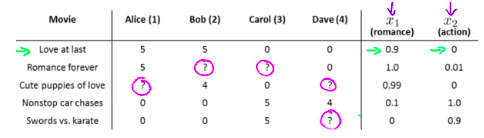
\includegraphics[width=\textwidth]{thesis/images/content_based_1.png}
\caption{Content-based Utility Matrix}
\end{figure}

Như ví dụ ở trên, ta đơn giản hóa bằng cách xây dựng vector đặc trưng cho mỗi bộ phim. Chiều thứ nhất của vector là độ lãng mạn (romance), chiều thứ 2 là mức độ hành động (action). Gọi các vector đặc trưng cho mỗi bộ phim là $x_1$, $x_2$, $x_3$, $x_4$, $x_5$ ta sẽ có giá trị mỗi vector là $x_1$ = [0.9, 0], $x_2$ = [1.0, 0.01], $x_3$ = [0.99, 0], $x_4$ = [0.1, 1.0], $x_5$ = [0, 0.9].

Tương tự, tính cách của mỗi người dùng cũng có thể được mô hình hóa dưới dạng tập các tham số $\theta$. Dữ liệu huấn luyện để xây dựng các mô hình $\theta$ là cặp item profile - rating tương ứng với các người dùng mà user đó đã đánh giá. Việc điền giá trị còn thiếu trong ma trận utility là dự đoán mức độ quan tâm khi áp dụng mô hình $\theta$ lên chúng. Đầu ra có thể viết dưới dạng f($\theta$,x). 

\subsection{Xây dựng hàm mất mát}
Giả sử số người dùng là N, số phim là M. Ma trận profile là X = [$x_1$, $x_2$,..., $x_m$] $ \in R_{d \times M}$ (d là số feature) và ma trận utility $Y \in R_{M \times N}$ Thành phần ở hàng thứ m, cột thứ n của Y là mức độ quan tâm của người dùng thứ n lên sản phẩm m mà hệ thống thu thập được. Giả sử tìm được 1 mô hình cho mỗi người dùng minh họa bởi vector $W_n \in R^d$ sao cho độ quan tâm có thể được tính theo công thức:
\begin{equation}
    y_{mn} = w^T_n x_m + b_n
\end{equation}

Xét user thứ n, coi training set là tập hợp các thành phần đã được điền của $y_n$, có thể xây dựng hàm mất mát tương tự như ridge regression:
\begin{equation}
    L_n(w_n,b_n)=\frac{1}{2s_n} \underset{m:r_{m n}}{\sum} (w^n x_m + b_n - y_{m n})^2 + 
    \frac{\lambda}{2s_n} \|w_n\|^2_2 
\end{equation}
trong đó, thành phần thứ hai là regularization và $\lambda$ là tham số dương, $s_n$ là số lượng các item mà user thứ n đã đánh giá.

Vì ở biểu thức trên $s_n$ là hằng số nên ta tập trung vào tối ưu phương trình đơn giản hơn dưới đây.
\begin{equation}
    \min \frac{1}{2} \underset{m:r_{m n}}{\sum} (w^n x_m + b_n - y_{m n})^2 + 
    \frac{\lambda}{2} \|w_n\|^2_2 
\end{equation}

Content-based recommendation system có điểm mạnh là không cần có data về những người dùng khác vì việc gợi ý chỉ tập trung vào từng người dùng. Điều này giúp cho việc scale lên một lượng user lớn trở nên dễ dàng hơn. Hơn nữa, model này có thể nắm bắt được sở thích của người dùng (VD thể loại phim hay xem, ca sĩ ưa thích, ...) và từ đó có thể gợi ích niche item mà ít người dùng thích.

Tuy nhiên, content-based recommendation system vẫn còn một số điểm yếu như sau. Vì phương pháp cần phải có feature của từng sản phẩm nên vẫn phụ thuộc vào độ chính xác của thông tin các feature này. Ngoài ra, model này chỉ có thể recommend dựa trên sở thích đã biết của người dùng. Nói cách khác, model này không thể gợi ý những sản phẩm nằm ngoài sở thích đã biết của người dùng.

% \newpage
\section{Collaborative filtering recommendation system}
\subsection{Giới thiệu}
Content-based recommendation system tuy có thể xây dựng mô hình cho mỗi user không phụ thuộc vào các user khác mà chỉ phụ thuộc vào profile của các item thì vẫn còn những nhược điểm là không tận dụng được thông tin từ các user khác và có lúc không thể xây dựng được profile cho mỗi item. Tiếp theo sẽ là phương pháp có thể giải quyết được 2 vấn đề này, đó là \gls{CF}.
\newline Phương pháp dự đoán cơ bản của CF là nếu user X và user Y rate n items gần giống nhau, hay có hành vi giống nhau (cùng xem nhiều loại phim, cùng mua nhiều loại sản phẩm, ...) thì sẽ đánh giá hay tương tác (xem, mua,...) với các sản phẩm khác giống nhau. 
\newline Phương pháp CF là dựa trên độ quan tâm của user tới item đã biết trước để có thể dự đoán được item mà user khác thích. Ví dụ, có danh sách gồm m user {u1, u2, ...um} và 1 danh sách n item {i1, i2, ... , im} và mỗi user ui có 1 danh sách các item Iui mà user đó đã rate (xem, mua, ...). Những giá trị này có thể là rating, số lần mua, số lần click, ... 
\newline Phương pháp CF gặp phải nhiều thử thách. Thuật toán CF cần phải có khả năng xử lý với bộ dữ liệu thưa (bộ dữ liệu mà nhiều user, nhiều item nhưng lại ít rating), có thể xử lý được khi số lượng user và item tăng, đáp ứng cho khoảng thời gian ngắn, và nhiều vấn đề khác.
\newline Điểm khác biệt lớn nhất giữa CF và content-based recommendation system là CF chỉ sử dụng rating của user cho item còn content-based recommendation system thì phụ thuộc vào feature của item để dự đoán. Cả 2 phương pháp đều có những giới hạn nhất định. Do vậy một số phương Hybrid CF cũng đã được phát triển như content-boosted CF hay Personality Diagnosis nhằm vượt qua được những giới hạn của mỗi phương pháp.

\subsection{Những vấn đề gặp phải của Collaborative Filtering}
\textbf{Data sparsity (Dữ liệu thưa)}. Trong thực tế, rất nhiều recommendation system phải xử lý 1 lượng item rất lớn. Utility matrix thường vô cùng thưa nên việc tối ưu hiệu năng của recommendation system là rất quan trọng. Đối với vấn đề này, có 1 phương pháp được áp dụng là phương pháp giảm số chiều dữ liệu ví dụ như Singular Value Decomposition (SVD), loại bỏ những user, item không tiêu biểu hay không cần thiết nhằm giảm số chiều của Utility matrix.

\textbf{Cold start}. Khi có user mới hay item mới vào trong hệ thống, chưa từng có lịch sử rating hay tương tác gì của user, item này, việc gợi ý item phù hợp user có thể trở nên khó khăn. Item mới không được recommend nếu không có ai đánh giá và user cũng không nhận được recommend tốt vì chưa có lịch sử rating hay mua bán gì. Giải pháp như Hybrid CF có thể hỗ trợ vấn đề này. Với những item chưa được rating hay mua bao giờ, nếu có được các feature của item, vẫn có thể recommend được cho người dùng. 

\textbf{Scalability}. Khi số lượng user và item tăng quá nhanh, phương pháp CF bình thường sẽ gặp phải vấn đề scalability, yêu cầu tính toán vượt quá mức có thể đáp ứng. Ví dụ như khi có hàng chục triệu user và hàng triệu item thì độ phức tạp của thuật toán CF là O(n) sẽ là quá lớn. Chưa nói đến việc các hệ thống cần phải phản hồi ngay lập tức để đưa ra gợi ý hợp lý. Phương pháp giảm số chiều dữ liệu như SVD có thể dùng để giải quyết vấn đề scalability tuy nhiên vẫn phải trải qua bước matrix factorization. Ngoài ra còn có phương pháp khác như clustering CF, phương pháp này giải quyết vấn đề bằng cách tìm user để đánh giá trong 1 cụm nhỏ có độ tương đồng cao thay vì trên toàn bộ database. 

\textbf{Gray Sheep}. Gray sheep nói đến những user có quan điểm không nhất quán, không tương đồng với nhóm user nào nên không có nhiều giá trị đối với collaborative filtering. Có phương pháp được áp dụng đến giải quyết vấn đề này là lấy trung bình có tỉ lệ của phương pháp content-based và CF. Tỉ lệ của content-based và CF sẽ được xác định tùy theo mỗi user, cho phép hệ thống tối ưu hóa việc kết hợp content-based và CF cho mỗi user, giúp giải quyết vấn đề gray sheep.

\textbf{Shilling Attacks}. Có nhiều trường hợp đánh giá item, họ đưa ra đánh giá rất tốt về item của họ và đánh giá xấu về những item của đối thủ. Để tối ưu được hệ thống CF thì cần tránh được vấn đề này. Phương pháp item-based CF cho thấy bị ít ảnh hưởng bởi shilling attack hơn là user-based CF. Ngoài ra phương pháp hybrid CF cũng là một giải pháp cho shilling attack vì ít bị phụ thuộc vào đánh giá của user khác hơn so với phương pháp CF đơn thuần.

\subsection{Neighbor-based Collaborative Filtering}
\subsubsection{Similarity Computation (Xác định độ giống nhau)}
Việc quan trọng nhất phải làm trong collaborative filtering là xác định được sự giống nhau (similarity) giữa 2 user hay 2 item. Ví dụ trong item-based CF, việc tính toán độ giống nhau giữa item i và item j là đầu tiên cần tìm ra những user đã đánh giá cả 2 item và áp dụng hàm tính toán độ giống nhau. Còn đối với user-based CF, tính toán độ giống nhau giữa 2 user u và user v mà đã cùng rate nhiều item. Những hàm tính toán độ giống nhau có những hàm như cosine similarity, euclidean distance, pearson correlation.
\newline Cosine similarity là hàm được sử dụng nhiều nhất. Công thức của cosine similarity là dưới đây:
\begin{equation}
    similarity = \cos{u_1, u_2} = \frac{u^T_1 u_2}{\|u^T_1\|.\|u_2\|}
\end{equation}
\newline Trong đó $u_{1,2}$ là vector tương ứng với user 1, 2 đã được chuẩn hóa.
\newline Độ similarity (giống nhau) của 2 vector là 1 số trong đoạn [-1, 1]. Giá trị bằng 1 thể hiện hai vector hoàn toàn similar với nhau. Hàm số cos của một góc bằng 1 nghĩa là góc giữa hai vector bằng 0, tức một vector bằng tích của một số dương với vector còn lại. Giá trị bằng -1 thể hiện hai vector này hoàn toàn trái ngược nhau. Điều này cũng hợp lý , tức khi hành vi của hai users là hoàn toàn ngược nhau thi similarity giữa hai vector đó là thấp nhất.

\subsubsection{Chuẩn hóa dữ liệu}
Khi thực hiện tính similarity, ta vẫn cần phải gán 1 giá trị tạm thời nào đó cho những ô rating trống trong Utility matrix. Nếu gán 0 thì không được vì giá trị quá thấp, sẽ giống như user ghét item đó, nếu gán trị trung bình ví dụ như 3 (đối với rating 1 đến 5) thì vẫn có thể gặp vấn đề như sau. Nếu với những user rating khắt khe, thường chỉ rating 1, 2, 3 thì giá trị 3 ở đây có thể là quá cao, còn với user dễ tính, thường rating 3, 4, 5 thì giá trị này là có thể là quá thấp. Do vậy, cần phải chuẩn hóa dữ liệu của Utility matrix.
\newline Bước đầu tiên của chuẩn hóa là tính trung bình các rating của người dùng. Giá trị này cao sẽ tương ứng với user dễ tính và ngược lại. Tiếp tục trừ từ mỗi rating đi giá trị này và thay giá trị chưa biết bằng không thì ta được Utility matrix đã chuẩn hóa. Bước chuẩn hóa này quan trọng cũng vì lý do sau đây. Thứ nhất, việc trừ đi trung bình cộng của mỗi cột khiến trong trong mỗi cột có những giá trị dương và âm. Những giá trị dương tương ứng với việc user thích item, những giá trị âm tương ứng với việc user không thích item. Những giá trị bằng 0 tương ứng với việc chưa xác định được liệu user có thích item hay không. Lý do thứ hai là vì số chiều của Utility matrix thường rất lớn, có thể lên tới hàng chục triệu user và hàng triệu item, việc lưu toàn bộ Utility matrix sẽ tốn rất nhiều bộ nhớ. Thấy rằng số lượng rating biết trước thường rất nhỏ so với kích thước của utility matrix nên cách tốt hơn là lưu dưới dạng sparse matrix, tức chỉ lưu giá trị khác không và vị trí của chúng. Tức là những rating chưa biết nên được thay bằng 0. Việc này giúp tối ưu bộ nhớ rất nhiều.

\subsubsection{Điền các giá trị khuyết trong utility matrix}
Việc dự đoán mức độ quan tâm (predict rating) của user với một item dựa trên các user giống với user này nhất rất giống với phương pháp k-nearest neighbors (KNN) với hàm khoảng cách là cosine similarity. Tương tự như KNN, neighbor-based CF cũng dùng thông tin của k user gần nhất để dự đoán. Để đánh giá độ quan tâm của user đối với 1 item, chỉ cần quan tâm tới các user lân cận đã từng đánh giá item đó. Tuy nhiên, trong KNN thì các distance là các khoảng cách không âm còn similarity trong neighbor-based thì có thể âm. Công thức dự đoán rating của user u cho item i là:
\begin{equation}
    \widehat{y_{i,u}} = \frac{\sum_{u_j \in N(u,i)} \overline{y_{i,u}} sim(u,u_j)}
                        {\sum_{u_j \in N(u,i)} |sim(u,u_j)|}
\end{equation}
Trong N(u, i) là tập hợp k user có similarity cao nhất với user u mà đã rate i.
Để quy đổi giá trị rating dự đoán về thang 5, cộng giá trị dự đoán với giá trị rating trung bình của mỗi user.
\newline Việc thực hiện recommend có thể thực hiện theo nhiều cách. Có thể sắp xếp những item chưa được rate theo giá trị giảm dần của rating dự đoán để recommend cho người dùng, hoặc recommend tất cả item có rate dự đoán đã chuẩn hóa lớn 0.

\subsubsection{Item-based collaborative filtering}
Phương pháp user-based vẫn còn 1 số hạn chế như sau. Đầu tiên là, số lượng user thường lớn hơn số lượng item rất nhiều. Do đó kích thước ma trận similarity là rất lớn. Việc lưu trữ ma trận nhiều khi không khả thi. Thứ hai là, utility matrix thường rất sparse và số lượng user lại rất lớn so với số lượng item dẫn đến nhiều cột của utility matrix có rất ít hoặc không có giá trị biết trước. Do đó, khi user thay đổi rating trước đó hay đánh giá thêm item, trung bình cộng rating hay vector chuẩn hóa thay đổi rất nhiều. Dẫn đến việc tính toán ma trận similarity, vốn đã tốn nhiều thời gian và bộ nhớ, cần phải thực hiện lại.
\newline Cách tiếp cận khác là thay vì tìm sự giống nhau giữa các user, chuyển sang tìm sự giống nhau giữa các item. Nếu user thích 1 item thì hệ thống nên gợi ý những item tương tự item đó cho user đó. Phương pháp này có những ưu điểm sau. Vì số item nhỏ hơn nhiều số item nên ma trận similarity nhỏ hơn rất nhiều giúp tính toán hiệu quả hơn. Thứ hai là vì số lượng item ít hơn user mà tổng rating không đổi, dẫn đến việc số rating item có được sẽ nhiều hơn số rating mà user rate. Từ đó dẫn đến việc tính độ similarity đáng tin cậy hơn, giá trị trung bình mỗi hàng thay đổi ít hơn khi có rating bị thay đổi dẫn tới việc cập nhật ma trận similarity được thực hiện ít hơn.

\subsubsection{Top-N recommendation}
Top-N recommendation là việc recommend 1 tập hợp gồm N item được xếp hạng mà user có thể thích. Ví dụ như khi sử dụng youtube, nếu user truy cập youtube với tài khoản youtube của mình, ở trang chủ, user sẽ được recommend 1 số video phù hợp với mỗi cá nhân. Phương pháp Top-N recommendation phân tích utility matrix để tìm ra sự liên hệ giữa các user hay item khác nhau và dựa trên đó tìm những gợi ý hợp lý. Ta có thể chia Top-N recommendation thành 2 phương pháp là user-based top-N recommendation và item-based top-N recommendation.
\newline Với phương pháp user-based top-N recommendation, bước đầu tiên là tìm ra k user giống nhất với user đang muốn được recommendation nhất. Sau khi đã tìm ra k user đó, những item đã được k user này đánh giá (mua, xem) được tập hợp thành 1 tập C. Trong tập C, những sản phẩm được rating cao hay xuất hiện nhiều mà user chưa mua sẽ được ưu tiên recommend.
\newline Còn với phương pháp item-based top-N recommendation, đầu tiên tìm tập k item giống nhất với mỗi item mà user đã mua. Sau đó tìm ra tập C bằng cách loại bỏ những item mà user đã mua ra khỏi tập k item giống nhất với các item đã mua. Những item còn lại sẽ được xếp hạng dựa trên độ giống của item với item mà người dùng đã mua.

\subsubsection{Lợi thế và khó khăn khi ứng dụng neighbor-based collaborative filtering}
Việc ứng dụng neighbor-based CF có những lơi thế khá rõ như dễ áp dụng, không phụ thuộc vào thông tin của item, không phải thực hiện công đoạn huấn luyện, ngoài ra so với phương pháp khác như content-based thì có độ chính xác cao hơn.

Tuy nhiên, phương pháp neighbor-based CF vì là phương pháp memory-based nên vẫn có vấn đề lớn về khả năng mở rộng (scalability). Khi mà số người dùng hay số item trở nên quá lớn, ma trận similarity sẽ tốn rất nhiều bộ nhớ. Hơn nữa, với số user hay item càng lớn thì việc tìm ra K hàng xóm gần nhất sẽ có cost rất lớn,

\subsection{Clustering collaborative filtering}
\subsubsection{Model-based CF}
Phương pháp neighbor-based CF ở trên là phương pháp memory-based CF. Phương pháp Memory-based CF sử dụng toàn bộ hay một phần của bộ dữ liệu để thực hiện việc dự đoán. Phương pháp này có một số ưu điểm như là dễ áp dụng, data mới có thể dễ dàng được thêm vào và sử dụng luôn để đánh giá. Tuy vậy memory-based CF vẫn còn một số nhược điểm như hiệu suất thâm khi bộ dữ liệu thưa và đặc biệt là ít có khả năng mở rộng quy mô khi gặp bộ dữ liệu quá lớn do tốn rất nhiều bộ nhớ. Những vấn đề này có thể được giải quyết với Model-based CF. Clustering CF là 1 trong những phương pháp tiếp cận của Model-based CF.

\subsubsection{Giới thiệu Clustering CF}
\noindent Nội dung dưới đây được đươc viết dựa theo tài liệu \cite{locnguyen2010modelbased}.
\newline Clustering \gls{CF} là hướng tiếp cận dựa trên bài toán phân tích ma trận thành phân tử (matrix factorization hoặc matrix decomposition). Clustering \gls{CF} dựa trên giả định rằng người dùng trong cùng một nhóm có cùng sở thích, vì vậy những người dùng này đánh giá các mặt hàng tương tự nhau. Do đó, người dùng được phân chia thành các nhóm được gọi là các cluster được định nghĩa là một nhóm người dùng tương tự nhau.
\newline Giả sử mỗi người dùng được biểu diễn dưới dạng vector xếp hạng ký hiệu $u_i$ = ($r_{i1}$, $r_{i2}$,..., $r_{in}$). Thước đo khác nhau giữa hai người dùng là khoảng cách giữa họ. Chúng ta có thể sử dụng khoảng cách Minkowski, khoảng cách Euclidian khoảng cách Manhattan hay độ tương đồng cosine.
$$ distance_{Minkowski}(u_1,u_2) = \sqrt[q]{\underset{j}{\sum}(r_{1j} - r_{2j})^q} $$
$$ distance_{Euclidian}(u_1,u_2) = \sqrt{\underset{j}{\sum}(r_{1j} - r_{2j})^2} $$
$$ distance_{Manhattan}(u_1,u_2) = \underset{j}{\sum}|r_{1j} - r_{2j}| $$
$$ similarity_{cosine} (u_1,u_2) = \cos{u_1, u_2} = \frac{u^T_1 u_2}{\|u^T_1\|.\|u_2\|} = \frac{\underset{j}{\sum}r_{1j} r_{2j}}{\sqrt{\underset{j}{\sum}r_{1j}^2} \sqrt{\underset{j}{\sum}r_{2j}^2}} $$

Khoảng cách giữa $u_1$ và $u_2$ càng ngắn hay độ tương đồng càng cao thì $u_1$ và $u_2$ càng giống nhau. Để thực hiện Clustering \gls{CF} cần thực hiện 2 bước sau:
\begin{itemize}
    \item Phân người dùng thành các cụm và mỗi cụm luôn chứa các giá trị đánh giá. Ví dụ, Mỗi cụm đều là kết quả từ thuật toán k-mean và một giá trị trung bình là vector đánh giá giống như vector người dùng.
    \item Người dùng cần được gợi ý được đưa vào một trong các cụm và đánh giá của người đó sẽ giống như đánh giá của cụm đó. Việc đưa người dùng vào cụm nào sẽ dựa trên khoảng cách của người dùng đới với cụm.
\end{itemize}
Vây nên bước quan trọng nhất là làm sao để phân người dùng vào các cụm. Có nhiều phương pháp clustering như k-mean và k-centroid. Phương pháp phổ biến nhất là k-mean, bao gồm 3 bước sau đây:
\begin{itemize}
    \item Ta chọn ngẫu nhiên k người dùng, mỗi người ban đầu đại diện cho tâm của một cụm. Từ đó, chúng ta có k tâm cụm. Mỗi tâm cụm này được coi là đại diện của người dùng của một cụm. Có tổng cộng k cụm.
    \item Đối với mỗi người dùng, khoảng cách giữa mỗi người dùng với k tâm cụm được tính toán. Người dùng đó sẽ thuộc về cụm gần nhất. Nói cách khác, nếu người dùng $u_i$ thuộc về cụm $c_v$, khoảng cách giữa $u_i$ và tâm $m_v$ của cụm $c_v$, được ký hiệu là $distance(u_i, m_v)$ là nhỏ nhất trong tất cả các cụm.
    \item Sau đó, tâm của tất cả các cụm được tính toán lại. Nếu điều kiện dừng được thỏa mãn thì dừng lại, nếu không thì lặp lại bước thứ 2.
\end{itemize}
Quá trình này được lặp lại cho đến khi điều kiện dừng được thỏa mãn. Có hai điều kiện dừng điển hình cho thuật toán k-mean:
\begin{itemize}
    \item k tâm của các cụm không thay đổi. Nói cách khác, k cụm không thay đổi. Điều kiện này thể hiện đã hoàn thành phân cụm.
    \item Cách khác là tiêu chí lỗi nhỏ hơn một ngưỡng được xác định trước.
\end{itemize}
Nếu như điều kiện dừng là tiêu chí lỗi nhỏ hơn một ngưỡng được xác định trước, tiêu chí lỗi sẽ được tính nhau sau:
$$ error = \underset{v=1}{\overset{k}{\sum}} \underset{u_i \in c_v}{\sum} distance(u_i,m_v) $$
Trong đó $c_v$ và $m_v$ lần lượt là cụm v và tâm của nó.

\subsubsection{Lợi thế và vấn đề gặp phải khi áp dụng Clustering Cf}
Phương pháp clustering CF có lợi thế như có thể dễ dàng áp dụng để chia bộ dữ liệu phức tạp thành nhiều cụm khác nha;, phù hợp cho bộ dữ liệu lớn; có tính linh hoạt cao, điều chỉnh tâm các cụm có thể thay đổi kết quả đầu ra; có thời gian chạy tuyến tính với số đối tượng.

Tuy nhiên clutering CF còn có một số vấn đề như không thể biết được số lượng cụm tối ưu do đó số cụm phải được chọn từ trước; nếu các cụm ban đầu được chọn ngẫu nhiên thì kết quả có thể thiếu tính nhất quán.

\subsection{Matrix factorization collaborative filtering}
\noindent Nội dung dưới đây được đươc viết dựa theo tài liệu \cite{machinelearningbasic}.
\subsubsection{Giới thiệu}
\gls{MFCF} là một hướng tiếp cận khác cho collaborative filtering dựa trên bài toán phân tích ma trận thành nhân tử (matrix factorization hoặc matrix decomposition). 

Trong content-based recommendation system, mỗi item đều có item profile, được mô tả bằng vector $x$. Ta cần tìm vector hệ số $w$ tương ứng với mỗi người dùng. Từ đó đánh giá của người dùng đó cho item xấp xỉ với:
$$ y \approx w^T x = x^T w $$
Khi đó ma trận utility sẽ xấp xỉ với:
$$ Y \approx X^T W $$
Trong content-based recommendation system, vector x được xây dựng dựa trên thông tin của item. Như vậy việc xây dựng item profile đóng vai trò quan trọng, ảnh hưởng trực tiếp đến hiệu năng của mô hình.

Giả sử, không cần phải xây dựng trước các vector x dựa trên thông tin item và vector này có thể được huấn luyện đồng thời với vector hệ số của mỗi người dùng. Có nghĩa là biến số trong bài toán tối ưu là cả X và W. X là man trận của toàn bộ item profile, mỗi cột tương ứng với một item, W là ma trận của toàn bộ vector hệ số của người dùng, mỗi cột tương ứng với một người dùng.

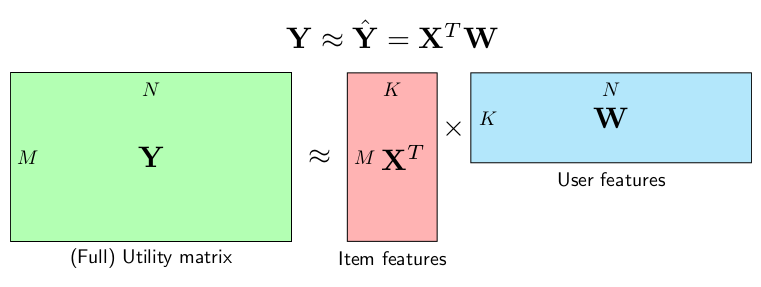
\includegraphics[width=\textwidth]{thesis/images/MFCF1.png}

Với cách làm này, ta cố gắng xấp xỉ ma trận utility $Y \in R^{M \times N}$ bằng tích của hai ma trận $ X \in R^{M \times K} $ và $ W \in R^{K \times N} $. Thông thường, K được chọn là số nhỏ hơn rất nhiều so với M, N. Khi đó, cả hai ma trận X và W đều có rank không vượt quá K. Do vậy, phương pháp này còn được gọi là low-rank matrix factorization. 

Ý tưởng đằng sau \gls{MFCF} chính là sự tồn tại của các tính chất ẩn mô tả sự liên quan giữa các item và người dùng. Ví dụ trong hệ thống gợi ý sách, những tính chất ẩn ở đây có thể là các thể loại sách trinh thám, lịch sử, giáo dục,... hoặc cũng có thể là kết hợp nào đó của các thể loại này. Mỗi item sẽ mang tính chất ẩn ở một mức độ nhất định nào đó, điều này sẽ được thể hiện ở vector x của item đó, hệ số này càng cao thể hiện item mang cần nhiều tính chất đó. Mỗi người dùng cũng tương tự như vậy. Mỗi người dùng có thể có sở thích đọc sách trinh thám, lịch sử, giáo dục,... hoặc thích thể loại được kết hợp bởi những thể loại này, điều này sẽ được thể hiện ở vector w của người dùng đó. Hệ số của 1 tính chất ẩn nào đó càng cao càng chứng tỏ người dùng càng thích item chứa nhiều tính chất ẩn đó. Từ đó giá trị $x^T w$ sẽ thể hiện được hứng thú của người dùng với item nhất định. Hệ số tính chất ẩn của item càng lớn và hệ số thể hiện độ thích của người dùng với tính chất đó càng lớn, giá trị trên sẽ càng lớn.
\section{Hybrid recommendation system}
(TODO)

Giới thiệu

Điểm mạnh, điểm yếu

Một số phương pháp


\section{Đánh giá recommendation system}
\subsection{Đánh giá rating dự đoán}
Độ chính xác của recommendation system có thể được kết luận dựa trên kết quả đánh giá. Việc đánh giá recommendation system tùy theo mỗi loại recommendation. Có 1 số phương pháp đánh giá như Mean Absolute Error (MAE), Normalized Mean Absolute Error (NMAE), Root Mean Squared Error (RMSE).

\subsubsection{Mean Absolute Error (MAE) và Normalized Mean Absolute Error (NMAE)}
Phương pháp được sử dụng tương đối phổ biến trong việc đánh giá recommendation system là MAE, tính toán trung bình của giá trị đối của hiệu giữa rating dự đoán và rating thực
\begin{equation}
    MAE = \frac{\sum_{\{i,j\}} |p_{i,j} - r_{i,j}|}{n}
\end{equation}
Trong đó n là tổng số rating của tất cả user, $p_{i,j}$ của user i đối với item j còn $r_{i,j}$ là giá trị rating thực của user i đối với item j. Giá trị MAE càng thấp chứng tỏ độ chính xác của dự đoán càng cao.
\newline Recommendation system khác có thể dùng một thang đo khác để đánh giá. Normalized Mean Absolute Error (NMAE) giúp tính ra xem error chiếm bao nhiêu phần trăm của toàn bộ thang đánh giá.
\begin{equation}
    NMAE = \frac{MAE}{r_{\max} - r_{\min}}
\end{equation}
$r_{\max}$ là giá trị lớn nhất và $r_{\min}$ là giá trị nhỏ nhất có thể đánh giá.

\subsubsection{Root Mean Squared Error (RMSE)}
Root Mean Squared Error (RMSE) trở nên nổi tiếng vì nó là phương pháp đánh giá cho gợi ý phim của Netflix prize
\begin{equation}
    RMSE = \sqrt{\frac{1}{n} \underset{\{i,j\}}{\sum}(p_{i,j} - r_{i,j})^2}
\end{equation}
Trong đó n là tổng số rating của tất cả user, $p_{i,j}$ của user i đối với item j còn $r_{i,j}$ là giá trị rating thực của user i đối với item j. 

\subsection{Đánh giá Top-N recommendation}
\subsubsection{Hit Rate}
Để đánh giá top N item gợi ý cho user, ta sử dụng hit rate. Mỗi khi user đánh giá 1 item trong top N item gợi ý, ta coi đó là 1 hit.
\newline Các bước tính ra hit rate của 1 user như sau. Đầu tiên, tìm tất cả những item mà user đã đánh giá. Sau đó loại bỏ đi 1 trong những item này (đây còn gọi là leave-one-out cross validation). Sử dụng tất cả những item còn lại để tìm ra top N recommendation. Nếu như item đã bị loại bỏ xuất hiện trong top N recommendation thì đó là 1 hit. 
Hit rate sẽ được tính bằng công thức sau.
\begin{equation}
    HR = \frac{total \: hit}{total \: user}
\end{equation}
Giá trị này cho thấy được tỉ lệ item đã bị loại bỏ xuất hiện trong top N gợi ý là bao nhiêu. Giá trị này càng cao chứng tỏ hệ thống Top-N recommendation càng tốt.
\newline Vấn đề của phương pháp này là khó để có thể gợi ý đúng 1 item duy nhất trong top N gợi ý. Do đó giá trị của hit rate với phương pháp leave-one-out cross validation thường khá nhỏ trừ phi có tập dữ liệu lớn.

\subsubsection{Rating Hit Rate (rHR)}
Một cách khác để tính hit rate là chia ra thành các hit rate của mỗi giá trị đánh giá. Những giá trị này cho thấy được những item được gợi ý được user thích đến mức độ nào vì mục đích của Top-N recommendation là gợi ý những item mà user thực sự thích. Vậy nên ở đây ta quan tâm đến những rating có giá trị cao hơn là rating có giá trị thấp.

\subsubsection{Cumulative Hit Rate (cHR)}
Vì ta chỉ quan tâm tới những rating cao, ta có thể bỏ qua rating thấp và chỉ tính toán hit rate của giá trị cao. Ví dụ như chỉ tính toán hit rate của của rating >= 4. Nếu gặp hit nhưng rating lại < 4 thì vẫn không được tính là hit.

\subsubsection{Average Reciprocal Hit Ranking (ARHR)}
Phương pháp này không chỉ tính hit rate mà còn đánh giá cả việc hit đó xuất hiện ở vị trí nào trong xếp hạng top N item được gợi ý. Hit ở vị trí càng cao trong bảng xếp hạng này thì có giá trị càng lớn. ARHR có thể được tính theo công thức sau đây.
\begin{equation}
    ARHR = \frac{\sum^n_{i=1} \frac{1}{rank_i}}{total \: user}
\end{equation}
Với $rank_i$ là vị trí của hit i trong top N recommendation. Ví dụ như 1 hit ở vị trí 1 sẽ có giá trị là 1 nhưng 1 hit ở vị trí 3 thì sẽ chỉ có giá trị là $\frac{1}{3}$.


\chapter{Sử dụng 3 phương pháp để xây dựng hệ thống gợi ý}
\section{Bài toán}
\subsection{Đặt vấn đề}
Hiện nay, ngành công nghệ thông tin đang ngày càng phát triển, kèm theo đó là sự phát triển của các dịch vụ online như youtube, netflix, amazon,... Và đối với những dịch vụ này, hệ gợi ý đóng vai trò vô cùng quan trọng trong các dịch vụ này. Chẳng hạn như Amazon khẳng định 35\% doanh thu của họ đến từ hệ thống gợi ý của dịch vụ này. Trong hệ gợi ý, 1 bài toán được sử dụng rất nhiều đó chính là Top-N recommendation.
\newline Bài toán này nhằm tìm ra N sản phẩm mà mỗi người dùng sẽ có xu hướng hứng thú nhất. Những ví dụ tiêu biểu của bài toán này là những video gợi ý cho người xem ở trang chủ youtube sau khi người dùng đăng nhập, những sản phẩm được gợi ý khi mua hàng trên amazon, những phim được gợi ý khi đăng nhập vào netflix,...
\newline Trong phần ứng dụng này, em sẽ triển khai hệ thống Top-N recommendation.

\subsection{Bài toán đặt ra}
Xây dựng một hệ thống Top-N recommendation gợi ý phim cho người dùng.
\section{Công cụ sử dụng}
\subsection{Môi trường phát triển}
\subsubsection{Google Colab}
Google colab là môi trường Jupyter Notebook miễn phí, không yêu cầu cài đặt và chạy hoàn toàn ở trên cloud. Sử dụng Google Colab, ta có thể thực thi viết và thực thi code, lưu và chia sẻ nghiên cứu, và có thể sử dụng nguồn tài nguyên tính toán mạnh.

Điểm mạnh của Google colab là đã tích hợp sẵn rất nhiều thư viện Python. Đối với người bắt đầu học python thì rất nhanh và tiện lợi do không cần cài đặt gì. Google colab cho phép sử dụng GPU miễn phí. Người dùng có thể thực thi code không bị gián đoạn trong 12 giờ liên tục, được sử dụng RAM lên tới 25GB. Notebook luôn được lưu ở trên google drive nên có thể chỉnh sửa, chia sẻ và thực thi ở mọi nơi.

Tuy vậy, Google colab vẫn có 1 điểm bất lợi như sau. Người dùng vẫn cần phải cài đặt tất cả thư viện không có sẵn và phải thực hiện điều này trong tất cả các session làm việc. Google drive luôn là nơi lấy dữ liệu và lưu trữ dữ liệu nhưng đôi khi cũng có thể là trên local, việc này có thể dẫn đến việc tiêu tốn bandwidth rất nhiều nên dataset lớn. Điểm bất lợi lớn nhất của Google colab là vì sử dụng data từ Google drive nên rất khó để sử dụng dataset quá lớn vì Google drive chỉ cung cấp 15 GB miễn phí.

\subsection{Dataset}
\subsubsection{MovieLens 100k}
Bộ dữ liệu MovieLens được thu thập bởi GroupLens Research Project tại đại học Minnesota.
Bộ dữ liệu này bao gồm 100.000 đánh giá (từ 1 đến 5) của 943 người dùng cho 1682 phim. Mỗi người dùng đều đã đánh giá ít nhất 20 phim và có thông tin cơ bản của người dùng như tuổi, giới tính, nghề nghiệp, mã zip.
\newline Dữ liệu được thu thập qua website MovieLens (movielens.umn.edu) trong khoảng thời gian 7 tháng từ 19/9/1997 đến 22/4/1998. Bộ dữ liệu này đã được xóa những người dùng có ít hơn 20 đánh giá hay những người dùng không có thông tin cơ bản cụ thể. 

\subsubsection{Goodbooks 10k}
Bộ dữ liệu này chứa đánh giá của người dùng cho mười nghìn cuốn sách phổ biến, với 6 triệu đánh giá. Nguồn của những đánh giá này được tìm thấy trên internet. Nói chung có khoảng 100 đánh giá cho mỗi cuốn sách, tuy nhiên một số có ít đánh giá hơn. Có thể đánh giá từ một đến năm.
\newline Cả ID sách và ID người dùng đều liền kề nhau. Đối với sách, chúng là 1 đến 10000, đối với người dùng là 1 đến 53424. Tất cả người dùng đã thực hiện ít nhất hai xếp hạng. Số xếp hạng trung bình cho mỗi người dùng là 8.
\newline Ngoài ra còn có dữ liệu những cuốn sách được đánh dấu để đọc bởi người dùng, thông tin cơ bản của sách như tác giả, năm,... và thể loại sách.

\section{Tiếp cận sử dụng phương pháp Neighbor-based CF}
\subsection{User-Based Top-N recommendation}
Phương pháp này dựa trên phương pháp user-based top-N recommendation ở trên nhưng đã được điều chỉnh để phù hợp cho bộ dữ liệu Movielens. Các bước thực hiện của phương pháp này như sau. Đầu tiên, tìm k user giống nhất cho active user sử dụng phương pháp cosine similarity. Sau đó, tìm set C bao gồm tất cả những item mà k user này đã đánh giá cùng với các rating của mỗi user cho mỗi item đó. Sau đó loại bỏ các item trùng nhau trong set C, những item còn lại sẽ gồm các giá trị trung bình rating của của những user trong k user cho những item này. Sau đó sắp xếp set C theo giá trị giảm dần của trung bình các rating. Lấy N giá trị đầu tiên ta có top-N recommendation.

\subsection{Item-Based Top-N recommendation}
Phương pháp này dựa trên phương pháp item-based top-N recommendation ở trên, đã được điều chỉnh để phù hợp cho bộ dữ liệu Movielens. Các bước thực hiện phương pháp này như sau. Đầu tiên, tìm k item giống nhất cho mỗi item dựa trên cách tính cosine similarity. Sau đó tìm set C, là hợp của các tập k item giống nhất với những item mà active user thích (có rating > 0 sau khi đã chuẩn hóa). Sau đó xóa những item mà active user và item bị trùng lặp, những item còn lại bao gồm các số lần xuất hiện trong set C. Sắp xếp set C theo giá trị xuất hiện giảm dần, lấy N item đầu tiên, ta được top-N recommendation.

\subsection{Top-N recommendation dựa trên rating dự đoán}
Phương pháp này là phương pháp tìm top-N recommendation cho active user dựa trên việc tính toán rating của active user đó cho tất cả các item. Bước đầu tiên của phương pháp này là áp dụng phương pháp user-based collaborative filtering để dự đoán rating của user đó cho mỗi item. Bước tiếp theo, tìm ra N item mới được dự đoán rating có giá trị rating lớn nhất, ta có được top-N recommendation. Tuy nhiên phương pháp này gặp vấn đề performance vì để tìm được top-N recommendation cho active user, cần phải dự đoán tất cả rating của user đó cho tất cả các item.
\section{Tiếp cận sử dụng phương pháp phân rã ma trận}
\input{thesis/chapters/problem/MF_CF}
\section{Tiếp cận sử dụng phương pháp clustering CF}
\input{thesis/chapters/problem/clustering_CF}
\chapter{Kết quả thực nghiệm và so sánh}
\input{thesis/chapters/problem/result}
% \chapter{Huấn luyện mạng nơ-ron trong nhiều môi trường học tăng cường}
\label{chap:problem_rl}
\section{Mô hình học tăng cường}
fomalization
\newpage
\section{Huấn luyện mạng nơ-ron để tối ưu hóa cách chơi}
optimal-policy
\newpage
\section{Môi trường đa nhiệm trong học tăng cường}
multitask-rl
\newpage
\section{Công việc liên quan}
related works
% \chapter{Tối ưu hóa đa nhiệm cho nhiều môi trường học tăng cường}
\label{chap:propose}

\section{Cách tiếp cận tiến hóa cho học tăng cường}
\subsection{Thuật toán tiến hóa trong học tăng cường}
evolution-rl
\newpage
\subsection{Điểm mạnh và điểm yếu của thuật toán tiến hóa trong học tăng cường}
strength-weaknesses
\newpage
\newpage
\section{Đa nhiệm trong học tăng cường}
\subsection{Khai thác các nhiệm vụ}
exploit
\newpage
\subsection{Độ hiệu quả}
effective
\newpage
\newpage
% \chapter{Kết quả thực nghiệm}
\label{chap:result}


\section{Cơ sở so sánh thuật toán tiến hóa}
baseline
\newpage
\section{Các bộ thực nghiệm}
\section{Mạng Nơ-Ron có cấu trúc}
\subsection{Bộ dữ liệu n-bit}
\subsection{Bộ dữ liệu UCI}

\newpage
\section{Các môi trường học tăng cường}
\subsection{Cart Pole}
\subsection{Bộ dữ liệu UCI}

\newpage
\section{Siêu tham số}
hyperparams
\newpage
\section{Cài đặt thực nghiệm}
config
\newpage
\section{Kết quả}

\subsection{Kết quả so sánh CEA, MFEA, MFEA-II}

  Tham số thực nghiệm mô hình: \\
$pop size: 90\\
numberiterations: 1000\\
sbxdi: 2\\
pmdi: 5\\
pswap: 0.5\\
dimension: 50\\
rmp: 0.3\\
repeat: 10\\
$

\begin{table}
	\caption{4-bit even parity problem}
    \begin{center}
    \begin{tabular}{|c|c|c|c|}
    \hline
    \multirow{1}{*}{\textbf{Method}} & \multicolumn{1}{c|}{\textbf{Subtask1}} & \multicolumn{1}{c|}{\textbf{Subtask 2}} & \multicolumn{1}{c|}{\textbf{Subtask 3}} \\ \hline
    CEA (4,5,6) & $0.0331 \pm 0.0091 $& $0.0166 \pm 0.0097$ & $\mathbf{0.0058 \pm 0.0012}$ \\ 
    MFEA (4,5,6) & $0.0268 \pm 0.0078$ & $\mathbf{0.0116 \pm 0.0034}$ & $0.0068 \pm 0.0016$ \\ 
    MFEAII (4,5,6)  & $\mathbf{0.0260 \pm 0.01}$ & $0.0163 \pm 0.0083$ & $0.0140 \pm 0.0106$ \\ \hline
    CEA (6,7,8) & $0.0115 \pm 0.0083$ & $0.0072 \pm 0.0064$ & $0.0026 \pm 0.0018$ \\ 
    MFEA (6,7,8) & $\mathbf{0.0082 \pm 0.0051}$ & $\mathbf{0.0029 \pm 0.0012}$ & $\mathbf{0.0012 \pm 0.0009}$ \\ 
    MFEAII (6,7,8)  & $0.0091 \pm 0.0066$ & $0.0038 \pm 0.0024$ & $0.0013 \pm 0.001$ \\ \hline
    
    \end{tabular}
    \end{center}
    
    \label{tab:result:nbit}
   
    \caption{6-bit even parity problem}
    \begin{center}
    \begin{tabular}{|c|c|c|c|}
    \hline
    \multirow{1}{*}{\textbf{Method}} & \multicolumn{1}{c|}{\textbf{Subtask1}} & \multicolumn{1}{c|}{\textbf{Subtask 2}} & \multicolumn{1}{c|}{\textbf{Subtask 3}} \\ \hline
    CEA (4,5,6) & $0.0514 \pm 0.0096$ & $0.0378 \pm 0.0091$ & $0.0279 \pm 0.0086$ \\ 
    MFEA (4,5,6) & $\mathbf{0.0457 \pm 0.0164}$ & $\mathbf{0.0323 \pm 0.0074}$ & $\mathbf{0.0245 \pm 0.0065}$ \\ 
    MFEAII (4,5,6)  & $0.0545 \pm 0.0161$ & $0.037 \pm 0.0102$ & $0.0333 \pm 0.0116$ \\ \hline
    CEA (5,6,7) & $\mathbf{0.0321 \pm 0.0077}$ & $0.0326 \pm 0.0088$ & $0.0267 \pm 0.0114$  \\ 
    MFEA (5,6,7) & $0.0379 \pm 0.013$ & $0.0288 \pm 0.01$ & $0.022 \pm 0.0078$ \\ 
    MFEAII (5,6,7)  &$ 0.0403 \pm 0.0114$ &$\mathbf{ 0.0283 \pm 0.01} $& $\mathbf{0.0197 \pm 0.0061}$ \\ \hline
    CEA (6,7,8) & $0.0298 \pm 0.012$ & $0.0219 \pm 0.0073$ & $0.0224 \pm 0.0061$ \\ 
    MFEA (6,7,8) & $\mathbf{0.0251 \pm 0.0085}$ & $\mathbf{0.0185 \pm 0.005}$ & $\mathbf{0.0143 \pm 0.0047}$ \\ 
    MFEAII (6,7,8)  &$ 0.0289 \pm 0.0066$ &$ 0.023 \pm 0.0079$ & $0.0193 \pm 0.0076$ \\ \hline
    
    \end{tabular}
    \end{center}
    
    \label{tab:result:nbit}
    
    \caption{8-bit even parity problem}
    \begin{center}
    \begin{tabular}{|c|c|c|c|}
    \hline
    \multirow{1}{*}{\textbf{Method}} & \multicolumn{1}{c|}{\textbf{Subtask1}} & \multicolumn{1}{c|}{\textbf{Subtask 2}} & \multicolumn{1}{c|}{\textbf{Subtask 3}} \\ \hline
    CEA (5,6,7) & $0.0524 \pm 0.0122$ & $0.0401 \pm 0.0118$ & $0.0424 \pm 0.0099$  \\ 
    MFEA (5,6,7) & $\mathbf{0.0502 \pm 0.0118}$ & $0.0377 \pm 0.008$ & $\mathbf{0.0288 \pm 0.0071}$ \\ 
    MFEAII (5,6,7)  & $0.0537 \pm 0.0108$ &$ \mathbf{0.0359 \pm 0.0066}$ &$ 0.0352 \pm 0.0085$ \\ \hline
    CEA (7,8,9) & $0.0334 \pm 0.0085$ & $0.0326 \pm 0.0086$ & $0.0244 \pm 0.0048$ \\ 
    MFEA (7,8,9) & $\mathbf{0.0323 \pm 0.0119}$ & $\mathbf{0.0237 \pm 0.0085}$ & $\mathbf{0.0196 \pm 0.0055}$ \\ 
    MFEAII (7,8,9)  & $0.0348 \pm 0.0088$ &$ 0.0303 \pm 0.0078$ &$ 0.0283 \pm 0.0083$ \\ \hline
    CEA (8,9,10)  & $0.0288 \pm 0.0067$ & $0.0331 \pm 0.0098$& $0.0259 \pm 0.0054$ \\ 
    MFEA (8,9,10)  & $0.0332 \pm 0.0122$ & $\mathbf{0.0230 \pm 0.0065}$ & $ 0.0252 \pm 0.0085$ \\ 
    MFEAII (8,9,10)  & $\mathbf{0.0282 \pm 0.0074}$ & $0.0270 \pm 0.0074$& $\mathbf{0.0223 \pm 0.0056}$ \\ \hline
    
    \end{tabular}
    \end{center}
    
    \label{tab:result:nbit}
\end{table}
\subsection{UCI Instances}
\begin{table}
    \begin{center}
    \begin{tabular}{|c|c|c|c|c|}
    \hline
    \multirow{1}{*}{\textbf{Instance}} & \multicolumn{1}{c|} {\textbf{Method}} & \multicolumn{1}{c|}{\textbf{Subtask1}} & \multicolumn{1}{c|}{\textbf{Subtask 2}} & \multicolumn{1}{c|}{\textbf{Subtask 3}} \\ \hline
    \multirow{3}{*} {breastCancer} & CEA   & $0.0066 \pm 0.0003$ & $0.0053 \pm 0.0005$ & $0.0044 \pm 0.0006$ \\ 
     & MFEA & $0.0067 \pm 0.0005$ & $0.0051 \pm 0.0005$ & $\mathbf{0.0044 \pm 0.0004}$ \\ 
    & MFEA II & $\mathbf{0.0066 \pm 0.0005}$ & $\mathbf{0.0051 \pm 0.0004}$ & $0.0046 \pm 0.0003$ \\ \hline
    \multirow{3}{*} {creditScreening} & CEA & $0.1239 \pm 0.0$ & $0.1239 \pm 0.0$ & $0.124 \pm 0.0001$ \\ 
   & MFEA & $0.1239 \pm 0.0$ & $0.1239 \pm 0.0$ & $0.1239 \pm 0.0001$ \\ 
   & MFEA II & $\mathbf{0.1239 \pm 0.0}$ & $\mathbf{0.1239 \pm 0.0}$ & $\mathbf{0.1239 \pm 0.0}$ \\ \hline
    \multirow{3}{*} {ionosphere} & CEA& $\mathbf{0.0022 \pm 0.0009}$ & $\mathbf{0.003 \pm 0.0009}$ & $0.0026 \pm 0.0011$ \\ 
    &MFEA & $0.0027 \pm 0.0008$ & $0.0033 \pm 0.0008$ & $0.0028 \pm 0.0005$ \\ 
    &MFEAII & $0.0024 \pm 0.0006$ & $0.0036 \pm 0.001$ & $\mathbf{0.0023 \pm 0.0007}$ \\ \hline
    \multirow{3}{*} {ticTacToe} & CEA & $\mathbf{0.0067 \pm 0.0018}$ & $0.007 \pm 0.0021$ & $0.0067 \pm 0.0016$ \\ 
    &MFEA & $0.0086 \pm 0.0022$ & $0.0087 \pm 0.0036$ & $0.0072 \pm 0.0027$ \\ 
    &MFEA II & $0.0083 \pm 0.0035$ & $\mathbf{0.007 \pm 0.0026}$ & $\mathbf{0.0062 \pm 0.0022}$ \\ \hline
    
    \end{tabular}
    \end{center}
    
    \label{tab:result:nbit}
    \caption{UCI problems}
\end{table}


\newpage


% \chapter*{Conclusion}
% \addcontentsline{toc}{chapter}{Kết Luận} this line

\newpage
\bibliographystyle{plain} % We choose the "plain" reference style
\bibliography{refs} % Entries are in the "refs.bib" file

\end{document}
